% Best Model Deep Dive, Equipo 03.
% Diseño: mismo tema Madrid y proporción 4:3 de slides.tex.
\documentclass{beamer}
\usepackage[utf8]{inputenc}
\usepackage[spanish,es-nodecimaldot,shorthands=off]{babel}
\usepackage{graphicx}
\usepackage{booktabs}
\usepackage{array}
\usetheme{Madrid}
\setbeamertemplate{navigation symbols}{}
\setbeamertemplate{blocks}[rounded][shadow=false]
\graphicspath{{figures/}{../02_outputs/figures/}}
\newcommand{\NTrain}{164.960}
\newcommand{\NTest}{66.168}
\newcommand{\NPobres}{33.024}
\newcommand{\TasaPobreza}{20,0\%}
\newcommand{\OcupadosPobres}{25,0\%}
\newcommand{\OcupadosNoPobres}{50,0\%}
\newcommand{\NBogota}{10.567}
\newcommand{\PorcBogota}{6,4\%}
\newcommand{\FoneCV}{0,768}
\newcommand{\PublicScore}{0,77}
\newcommand{\UmbralBest}{0,394}
\newcommand{\PrecisionBest}{74,4\%}
\newcommand{\RecallBest}{79,4\%}
\newcommand{\AucBest}{0,957}
\newcommand{\TPBest}{26.236}
\newcommand{\FNBest}{6.788}
\newcommand{\FPBest}{9.027}
\newcommand{\TNBest}{122.909}
\newcommand{\Leakage}{25,6\%}
\newcommand{\Undercoverage}{20,6\%}
\newcommand{\AccBase}{79,98\%}
\newcommand{\FoneBase}{0,00}
\newcommand{\SensBase}{0\%}
\newcommand{\EspBase}{100\%}
\newcommand{\FoneXgb}{0,762}

\title[Predicción de pobreza]{Predicción de pobreza en Colombia}
\subtitle{Best Model Deep Dive}
\author[Equipo 03]{Andrés Silva, Valentina Vera \& Julián Herrera}
\institute[Uniandes]{Universidad de los Andes}
\date[2026-20]{MECA 4107, 2026-20}
\newcommand{\fuente}[1]{\vfill{\fontsize{6.5}{7.5}\selectfont\color{black!65}#1\par}}
\newcommand{\cierre}[1]{\begin{block}{}\centering\small #1\end{block}}
\setlength{\tabcolsep}{5pt}
\renewcommand{\arraystretch}{1.18}
\newcolumntype{L}[1]{>{\raggedright\arraybackslash}p{#1}}

\begin{document}

% 01. Overview obligatorio.
\begin{frame}{LightGBM: el modelo ganador}
\framesubtitle{Best Model Overview}
\begin{columns}[T,onlytextwidth]
\begin{column}{0.40\textwidth}
\begin{block}{F1 público en Kaggle}
\centering
{\fontsize{34}{36}\selectfont\PublicScore}\par
\smallskip
{\small F1 en CV: \textbf{\FoneCV}}
\end{block}
\end{column}
\begin{column}{0.55\textwidth}
\small
\begin{tabular}{@{}ll@{}}
\textbf{Modelo} & LightGBM (GBDT)\\
Predictores & 1.296 variables, X7\\
Hojas / rondas & 31 / 748\\
Aprendizaje & 0,04\\
Validación & 5 folds estratificados\\
Umbral & \UmbralBest
\end{tabular}
\end{column}
\end{columns}
\medskip
\small
\textbf{Tres hallazgos para leer el resultado}
\begin{itemize}
\setlength{\itemsep}{0.2em}
\item Vivienda y mercado laboral concentran la señal predictiva.
\item Las relaciones observadas contienen curvaturas y umbrales.
\item Aún queda fuera el \textbf{\Undercoverage} de los hogares pobres.
\end{itemize}
\fuente{Equipo 03. Fuentes: registro de modelos, puntajes públicos de Kaggle y artifact de importancia.}
\note{El puntaje público localmente registrado corresponde al envío del 25 de octubre de 2026. F1 CV: 0,768403942. El umbral es 0,393939393939394. La subcobertura usa los errores OOF registrados; no corresponde a las etiquetas ocultas de Kaggle.}
\end{frame}

% 02. Dimensionalidad e interpretación.
\begin{frame}{1.296 predictores: cómo interpretarlos}
\small
Agregamos información del hogar y de sus miembros en \textbf{1.296 variables derivadas}.
\medskip
\begin{columns}[T,onlytextwidth]
\begin{column}{0.44\textwidth}
\textbf{El costo de esa riqueza}
\begin{itemize}
\setlength{\itemsep}{0.6em}
\item Medidas redundantes.
\item Interacciones difíciles de leer.
\item Menor interpretación directa.
\end{itemize}
\end{column}
\begin{column}{0.52\textwidth}
\textbf{Una ruta para entenderla}
\begin{enumerate}
\setlength{\itemsep}{0.6em}
\item \textbf{Permutar:} cuánto cae el F1.
\item \textbf{Describir:} cómo cambia la pobreza.
\item \textbf{Contrastar:} balance entre muestras.
\end{enumerate}
\end{column}
\end{columns}
\cierre{Podemos interpretar la predicción sin atribuirle efectos causales.}
\fuente{Construcción de X7 y análisis descriptivo del proyecto. Una variable derivada no equivale a una pregunta de encuesta.}
\note{X7 combina características del hogar, agregados por grupos de miembros, proporciones por categoría y medidas de personas concretas. La correlación puede repartir la importancia. Las curvas describen asociaciones marginales: no son efectos causales ni efectos parciales del modelo.}
\end{frame}

% 03. Ranking a la izquierda, mecanismos a la derecha.
\begin{frame}{Qué variables aportan más señal}
\begin{columns}[c,onlytextwidth]
\begin{column}{0.57\textwidth}
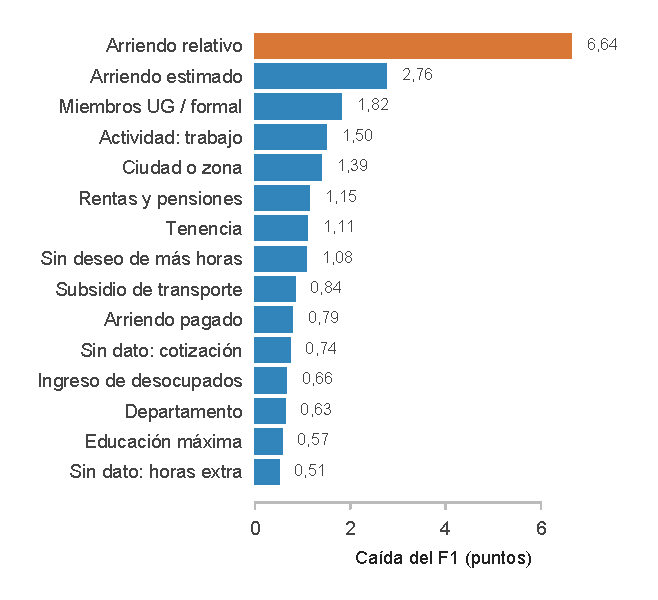
\includegraphics[width=\linewidth]{best_importancia_top15.pdf}
\end{column}
\begin{column}{0.39\textwidth}
\small
\textbf{Lectura económica}
\begin{itemize}
\setlength{\itemsep}{0.9em}
\item \textbf{Vivienda:} recursos y valor locativo.
\item \textbf{Formalidad:} estabilidad y protección.
\item \textbf{Composición:} ingresos que se reparten.
\end{itemize}
\medskip
{\footnotesize Más caída del F1 implica mayor dependencia predictiva.}
\end{column}
\end{columns}
\fuente{Permutación: promedio de 3 repeticiones, 5 folds y unos 2.000 hogares de validación por fold. Caídas en puntos de F1; no son efectos causales ni contribuciones aditivas.}
\note{El primer predictor divide el arriendo pagado o estimado entre miembros UG y línea de pobreza. El tercero usa miembros UG por ocupado formal. Arriendo relativo: caída de 6,64 puntos; arriendo estimado: 2,76; miembros por formal: 1,82. Las categorías sin dato pueden reflejar saltos del cuestionario, no ausencia de cotización ni de horas extra. La importancia se estima en submuestras de validación, no es una descomposición del F1 OOF completo.}
\end{frame}

% 04. Una sola conclusión, centrada.
\begin{frame}
\vfill
\begin{center}
{\usebeamercolor[fg]{structure}\LARGE
La señal de pobreza se concentra\\[0.35em]
en la vivienda y en la\\[0.35em]
capacidad laboral del hogar.}
\end{center}
\vfill
\note{Síntesis del ranking de importancia por permutación. No afirma causalidad ni que el resto de predictores sea prescindible sin volver a validar.}
\end{frame}

% 05. Selección original por mayor cambio al excluir Bogotá.
\begin{frame}{Bogotá y las diferencias entre muestras}
\begin{columns}[c,onlytextwidth]
\begin{column}{0.60\textwidth}
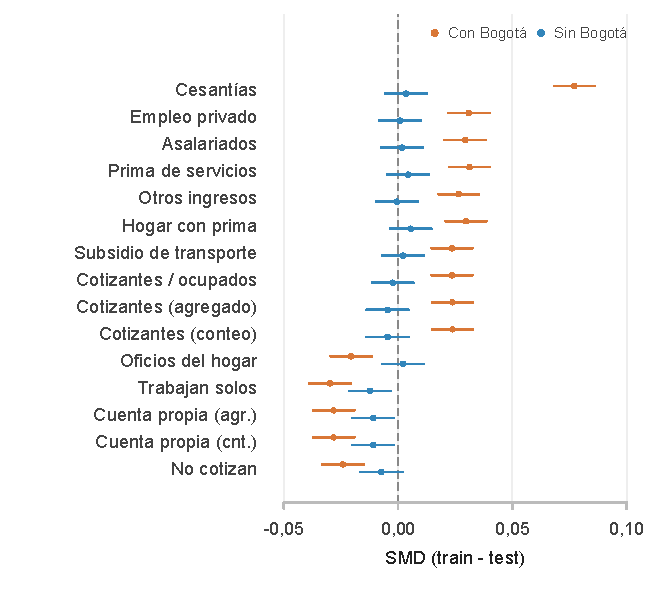
\includegraphics[width=\linewidth]{best_balance_original.pdf}
\end{column}
\begin{column}{0.36\textwidth}
\small
\begin{itemize}
\setlength{\itemsep}{0.8em}
\item Bogotá pesa \textbf{\PorcBogota} en train y no aparece en test.
\item Empleo formal y prestaciones muestran los mayores cambios.
\item Excluirla acerca varias medias; no garantiza mejor predicción.
\end{itemize}
\end{column}
\end{columns}
\fuente{Comparación original del script 04: 15 variables con mayor cambio en el valor absoluto del SMD al excluir Bogotá. Diferencia estandarizada train -- test e IC del 95\%.}
\note{No es una comparación directa Bogotá contra resto. Cada fila compara train con test, incluyendo o excluyendo Bogotá en train. La selección replica el cambio en el SMD absoluto; no es el ranking de importancia. El balance marginal no demuestra invariancia de la relación entre predictores y pobreza.}
\end{frame}

% 06. Asignar a todos a No pobre.
\begin{frame}{El desbalance y un clasificador ingenuo}
\begin{columns}[c,onlytextwidth]
\begin{column}{0.50\textwidth}
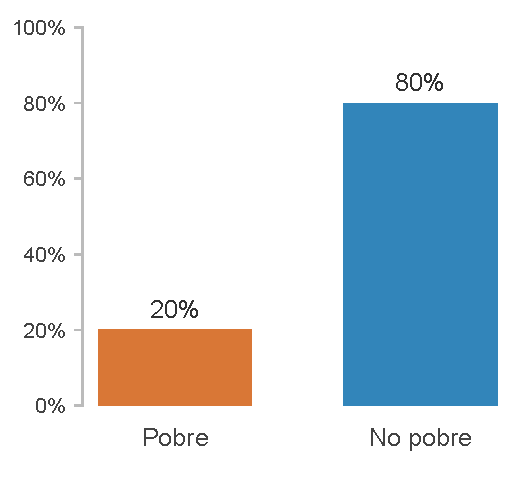
\includegraphics[width=\linewidth]{best_distribucion_clase.pdf}
\centering{\footnotesize Train: \NTrain{} hogares}
\end{column}
\begin{column}{0.45\textwidth}
\small
\textbf{Clasificar a todos como no pobres}
\medskip

\begin{tabular}{@{}lr@{}}
\toprule
Exactitud & \AccBase\\
\textbf{F1} & \textbf{\FoneBase}\\
Sensibilidad & \SensBase\\
Especificidad & \EspBase\\
\bottomrule
\end{tabular}
\medskip

No identificaríamos a ningún hogar pobre.
\end{column}
\end{columns}
\fuente{Distribución de Pobre en train. Clase positiva: hogar pobre. Métricas de asignar a todos a No pobre, sin entrenar un modelo.}
\note{El 20,0194 por ciento es pobre. Asignar todos a no pobres produce 131.936 TN y 33.024 FN. F1 y sensibilidad son cero; exactitud: 79,9806 por ciento. No se muestra precisión positiva porque no hay predicciones positivas.}
\end{frame}

% 07. Cuatro formas, sin logit.
\begin{frame}{Forma funcional de los principales predictores}
\centering
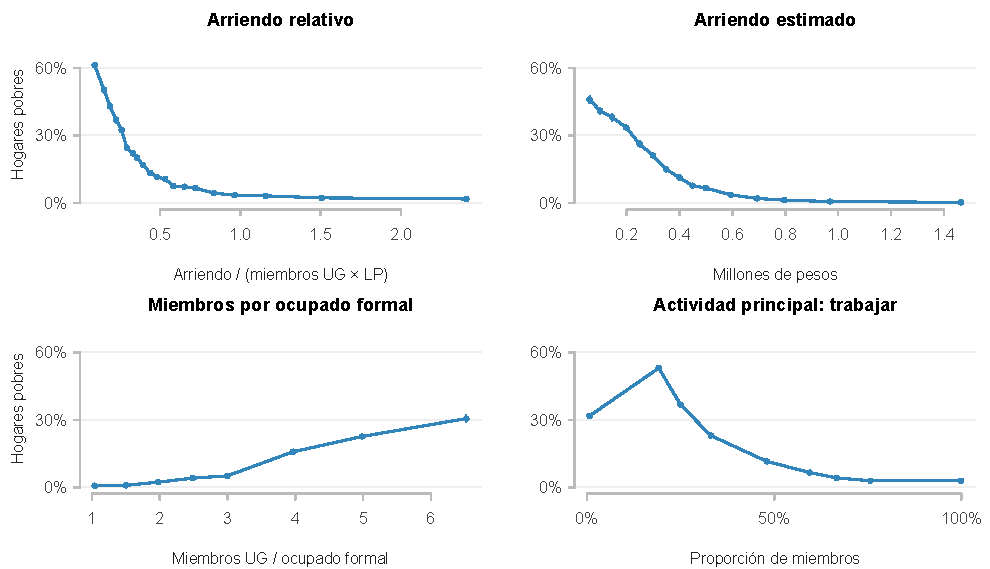
\includegraphics[width=0.98\textwidth]{best_datos_curvas.pdf}
\smallskip

{\small Las curvaturas y los umbrales observados motivan una especificación flexible.}
\fuente{Cuatro primeros del ranking. Tasas por grupos de cuantiles, IC de Wilson del 95\%, casos válidos y rango P1--P99. UG: unidad de gasto; LP: línea de pobreza.}
\note{Solo tasas observadas e intervalos. No se ajusta ni dibuja logit. Arriendo relativo y estimado se asocian negativamente con pobreza; miembros por formal, positivamente; la proporción cuya actividad principal es trabajar no es estrictamente monótona. Son asociaciones descriptivas, no PDP ni efectos causales. No prueban superioridad frente a un logit con transformaciones o a otro algoritmo de árboles. El cociente por formal excluye denominadores no válidos.}
\end{frame}

% 08. Configuración documentada y validación.
\begin{frame}{Por qué LightGBM se ajusta a estos patrones}
\small
\begin{tabular}{@{}L{0.36\textwidth}L{0.57\textwidth}@{}}
\toprule
\textbf{Desafío} & \textbf{Configuración seleccionada}\\
\midrule
Curvaturas e interacciones & Árboles: 31 hojas y 748 rondas\\[0.5em]
Muchas variables y sobreajuste & 100 casos por hoja; L1/L2 = 0,1/10\\[0.5em]
Control del aprendizaje & Tasa 0,04; 85\% de filas y variables\\[0.5em]
Clase pobre minoritaria & Umbral \UmbralBest{} elegido por F1 OOF\\
\bottomrule
\end{tabular}
\medskip

Con X7 y cinco folds: \textbf{LightGBM \FoneCV} frente a \textbf{XGBoost \FoneXgb}.
\cierre{La flexibilidad motiva el modelo; el F1 de validación respalda su selección.}
\fuente{Configuración y resultados del script 11. Se documenta búsqueda de 100 umbrales; no se conserva una bitácora de búsqueda de hiperparámetros de LightGBM.}
\note{La configuración se mantiene fija entre X5, X6 y X7. El umbral se optimiza sobre las mismas predicciones OOF usadas para reportar F1: no es validación anidada. Se entrena con log-loss. XGBoost también representa no linealidades e interacciones; la comparación empírica distingue los dos. La regularización controla el riesgo de sobreajuste, sin garantizar eliminarlo ni resolver las diferencias territoriales. F1 tampoco incorpora por sí solo costos sociales asimétricos.}
\end{frame}

% 09. Ranking del ganador, con Bogotá en el entrenamiento.
\begin{frame}{El ganador sí se entrenó con Bogotá}
\begin{columns}[c,onlytextwidth]
\begin{column}{0.60\textwidth}
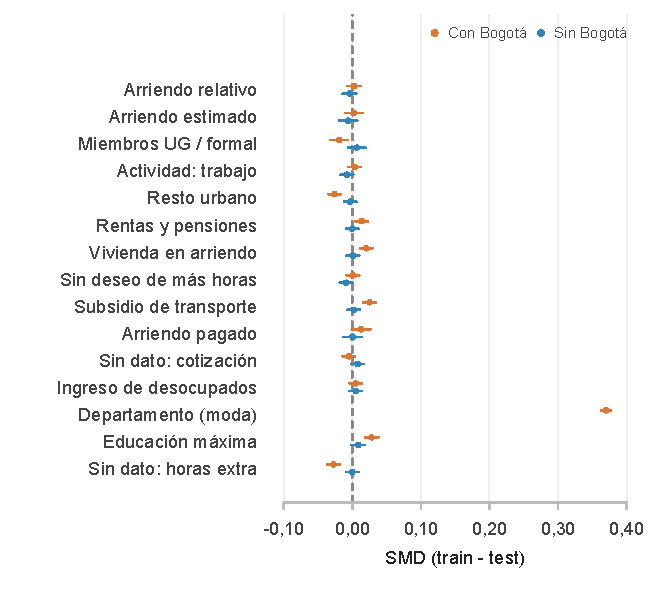
\includegraphics[width=\linewidth]{best_balance_bogota.pdf}
\end{column}
\begin{column}{0.36\textwidth}
\small
\begin{itemize}
\setlength{\itemsep}{0.8em}
\item Se conservaron los \textbf{\NBogota{} hogares} de Bogotá.
\item La mayoría de variables clave tiene brechas pequeñas.
\item Departamento conserva una diferencia territorial.
\end{itemize}
\end{column}
\end{columns}
\fuente{15 principales del LightGBM; SMD train -- test e IC del 95\%. Categóricas: indicador modal. El SMD de departamento sin Bogotá no se define por varianza nula.}
\note{Esta figura cambia la selección de la anterior: usa importancia por permutación. El ganador entrenó con Bogotá; este diagnóstico no implica reentrenamiento ni evaluación sin ella. Dominio es indicador de RESTO URBANO; tenencia, de arriendo. Departamento usa el indicador modal del artifact: SMD con Bogotá aproximadamente 0,370 y sin Bogotá indefinido, no cero. Conservar Bogotá requiere evaluar desempeño territorial; el balance solo no basta.}
\end{frame}

% 10. Diagnóstico con conteos reconstruidos y verificados.
\begin{frame}{Diagnóstico del modelo ganador}
\begin{columns}[c,onlytextwidth]
\begin{column}{0.56\textwidth}
\small
\textbf{Realidad}
\medskip

\begin{tabular}{@{}lrr@{}}
\toprule
Predicción & Pobre & No pobre\\
\midrule
Pobre & \textbf{\TPBest} & \FPBest\\
No pobre & \FNBest & \textbf{\TNBest}\\
\bottomrule
\end{tabular}
\medskip

{\footnotesize Umbral \UmbralBest; predicciones OOF.}
\end{column}
\begin{column}{0.39\textwidth}
\small
\begin{tabular}{@{}lr@{}}
\toprule
Precisión & \PrecisionBest\\
Sensibilidad & \RecallBest\\
\textbf{F1} & \textbf{\FoneCV}\\
AUC ROC & \AucBest\\
\bottomrule
\end{tabular}
\end{column}
\end{columns}
\cierre{La mejora predictiva convive con \FNBest{} hogares pobres que quedan fuera.}
\fuente{Registro de modelos. Conteos enteros reconstruidos de precisión y sensibilidad OOF y del total por clase; reproducen el F1 registrado.}
\note{TP = 26.236; FN = 6.788; FP = 9.027; TN = 122.909. No provienen de un archivo nuevo de predicciones OOF. El script verifica precisión y F1 con tolerancia 1e-10. El umbral se elige y evalúa con las mismas OOF: posible optimismo de selección. No son métricas separadas del test de Kaggle.}
\end{frame}

% 11. Consecuencias de los errores y decisión del umbral.
\begin{frame}{Filtración y subcobertura}
\begin{columns}[T,onlytextwidth]
\begin{column}{0.47\textwidth}
\begin{block}{Filtración}
\centering{\LARGE\Leakage}\par
\smallskip
{\small de los seleccionados no son pobres}
\end{block}
\small
\FPBest{} falsos positivos: recursos que llegan a hogares no pobres.
\end{column}
\begin{column}{0.47\textwidth}
\begin{block}{Subcobertura}
\centering{\LARGE\Undercoverage}\par
\smallskip
{\small de los pobres quedan fuera}
\end{block}
\small
\FNBest{} falsos negativos: hogares pobres excluidos del beneficio.
\end{column}
\end{columns}
\medskip
\small
Bajar el umbral amplía cobertura y puede aumentar la filtración; subirlo restringe el acceso.
\fuente{Diagnóstico OOF: filtración = FP/(TP+FP); subcobertura = FN/(TP+FN). Los denominadores representan poblaciones distintas.}
\note{Filtración es 1 menos precisión; subcobertura, 1 menos sensibilidad. Filtración no es la tasa de falsos positivos entre no pobres (6,84 por ciento). Bajar el umbral reduce o mantiene FN y aumenta o mantiene FP; la proporción de filtración no tiene monotonicidad garantizada en la muestra. Maximizar F1 no incorpora presupuesto, severidad de pobreza ni costos sociales asimétricos.}
\end{frame}

% 12. Viabilidad y cierre.
\begin{frame}{Condiciones para una política real}
\small
\begin{tabular}{@{}L{0.33\textwidth}L{0.59\textwidth}@{}}
\toprule
\textbf{Pregunta} & \textbf{Condición antes de desplegar}\\
\midrule
¿Encuesta corta? & Recoger vivienda, composición y trabajo de los miembros; validar una versión reducida.\\[0.6em]
¿Datos disponibles a tiempo? & Revisar ayudas y afiliación subsidiada: posible circularidad con la focalización vigente.\\[0.6em]
¿Funciona fuera de la muestra? & Validar por territorio y período; definir umbral según presupuesto y costo de excluir.\\
\bottomrule
\end{tabular}
\cierre{Es un candidato para apoyar la focalización, sujeto a validación operativa y territorial.}
\fuente{Diseño de X7 y diagnósticos del proyecto. El desempeño de una encuesta reducida aún no se ha validado.}
\note{1.296 predictores no son 1.296 preguntas: hay muchos agregados de las mismas respuestas. Trabajo y formalidad requieren información de los miembros. P6100 y P7510s3 incluyen régimen subsidiado y ayudas institucionales: no se afirma filtración directa del objetivo, pero usar asignaciones vigentes puede reproducir reglas previas o introducir información no disponible al desplegar. Se excluye el ingreso objetivo directo. Antes del despliegue: versión reducida validada, disponibilidad temporal, validación geográfica y temporal, calibración si se usan probabilidades como riesgo, y costos y presupuesto explícitos.}
\end{frame}

\end{document}
